\documentclass[11pt]{ctexart}         %编辑中文文档
\usepackage{amsmath,amsfonts,amssymb} %数学工具包
\usepackage[margin=1in]{geometry}     %页面设置,边距,页幅大小等
\usepackage{enumerate}                %有序列表工具包
%\usepackage{hyperref}                 %方便设置超链接
\usepackage{fancyhdr}                 %设置页眉页脚
\usepackage{float}                    %设置图片环绕样式
\usepackage{graphicx}                 %插入图片
\usepackage{color}
\usepackage{xcolor}
\usepackage{adjustbox}
\usepackage{pifont}
\usepackage{extarrows}
\usepackage{enumitem}
\usepackage{setspace}
\usepackage{subfigure}

\CTEXsetup[format={\Large\bfseries}]{section} %设置section标题左对齐,挺迷的
\usepackage[
	pdfstartview=FitH,
	CJKbookmarks=true,
	bookmarksnumbered=true,
	bookmarksopen=true,
	colorlinks,
	pdfborder=001,
	linkcolor=blue,
	anchorcolor=blue,
	citecolor=blue,
]{hyperref}
\hypersetup{hidelinks} %去除目录项以及超链接的方框

\pagestyle{fancy}                     %设置页眉页脚
\fancyhead{}                          %清除默认页眉
\fancyfoot{}                          %清除默认页脚
\fancyhead[L]{\slshape{Convex Optimization}}%设置自定义页眉左侧,slshape表斜体	
\fancyhead[R]{\slshape Chapter3 Convex Function}	
\fancyfoot[C]{\thepage}
\parindent 0ex %latex首段不缩进,其后段落缩进,\parindent为其后段落缩进的长度
\setlength{\parskip}{1em}  %段落间距
\renewcommand{\baselinestretch}{1.5}  %设置行距
\renewcommand{\vec}[1]{\boldsymbol{#1}}  %设置粗体向量
\newcommand{\tabincell}[2]{\begin{tabular}{@{}#1@{}}#2\end{tabular}}%表格内换行

\newenvironment{myenumerate}{\begin{enumerate}[itemsep=0pt,parsep=0pt,topsep=0pt]}{\end{enumerate}}
\newcommand{\liset}{itemsep=0pt,parsep=0pt,topsep=0pt}
\newcommand{\rebacklinespread}[1][-12pt]{\vspace{#1}}
\newcommand{\oneline}[1][12pt]{\vspace{#1}}
\newcommand{\premise}[1][dom\ f]{\forall\ x,y\in #1,\ \theta\in [0,1]}
\newcommand{\linearcombine}[2]{\theta #1+(1-\theta)#2}
\newcommand{\ii}{\,\in\,}
\newcommand{\dom}[1]{$dom\ #1$}
\newcommand{\rs}[2][R]{#1^{#2}} %Rspace or matrix space
\newcommand{\rl}[2][R]{#1_{#2}} %Rlimit or matrix space
\newcommand{\rls}[3][R]{#1_{#2}^{#3}} %R limit space or matrix limit space

\newcommand{\trans}[1]{#1^T#1} %transpose
\newcommand{\ftrans}[1]{\left(#1\right)^T#1} %fraction transpose

\newcommand{\ba}[1]{\begin{align*}#1\end{align*}}
\newcommand{\bc}[1]{\begin{cases}#1\end{cases}}
\newcommand{\li}[3][例]{
	#1:#2\\ 
	\phantom{#1:}\begin{minipage}[t]{0.9\linewidth}%注意这里phantom和minipage之间不能换行
	\setlength\parskip{12pt}
	#3
	\end{minipage}
	\oneline}
\newcommand{\sune}{\parbox{1em}{$ \Rightarrow $\\ [-10pt] $ \nLeftarrow $}} % Sufficiently unnecessary
\newcommand{\usne}{\parbox{1em}{$ \nRightarrow $\\ [-10pt] $ \Leftarrow $}} % unsufficiently necessary
\newcommand{\paint}[2][red]{{\color{#1}#2}} %着色



\begin{document}
\hrule height 4pt
\begin{Large}
	\textbf{Essence of the lecture (9(缺)/10/11)}\\
\end{Large}
\begin{large}
	\textbf{凸函数的性质:} 
\end{large}
\vspace{-16pt}
\begin{itemize} \setlength{\itemsep}{0pt}
	% 使用\displaystyle来解决行内时bigcap变形
	\item 凸函数的第一定义
	\item 凸函数的第二定义
	\item 凸函数的扩展
	\item 凸函数的第三定义:一阶条件
	\item 凸函数的第四定义:二阶条件
\end{itemize}
% 设置hrule的宽度为4pt
\hrule height 4pt
\textbf{凸函数的第一定义}\\
凸函数:f是凸函数,当且仅当其定义域为凸集,\\
\phantom{凸函数:}且$\forall x,y\in S,\ \forall \theta\in[0,1],\ f(\theta x+(1-\theta)y)\leq \theta f(x)+(1-\theta)f(y)$\\
严格凸函数:定义域为凸集,且$\forall x,y\in S,\ \forall \theta\in[0,1],\ f(\theta x+(1-\theta)y)< \theta f(x)+(1-\theta)f(y)$\\
类似定义有凹函数和严格凹函数

\textbf{凸函数的第二定义}\\
$f:\ R^n\to R$为凸函数$\Leftrightarrow dom\ f$为凸,且$\forall\ x\in dom\ f,\ \forall\ v,\ g(t)=f(x+tv)$为凸函数,$dom\ g=\{t\mid x+tv\in dom\ f\}$【g(t)是关于t的函数,相当于从高维降到一维,可以通过证明该一维函数g(t)为凸来证明高维的f(x)为凸】

\textbf{凸函数的扩展}\\
$f:\ R^n\to R$为凸函数,$dom\ f:\ C\subseteq R^n$\\ [8pt]
$
\tilde{f}=
\begin{cases}
	f(x) \quad &x\in dom\ f\\
	\infty\quad &x\notin dom\ f
\end{cases}
$,$\tilde{f}:\ R^n\to R$,$dom\ \tilde{f}:\ R$,即将f的定义域由C扩展到R
\vspace{16pt}

示性函数是凸函数,凸集$C\subseteq R^n$,同理将定义域由C扩展到$R^n$\\ [8pt]
$I_c(x)=\begin{cases}
	\infty\quad &x\notin C\\
	0\quad &x\in C
\end{cases}$,
注意$x\notin C$时,取值必须为$\infty$,否则总能够找到特定的值使其非凸非凹

\pagebreak
\begin{large}
	\textbf{凸函数的一阶条件}\\
\end{large}
设$f:\ R^n\to R$可微(这表示$dom\ f$一定是开集,因为对于扩展的$\tilde{f}$,其边界不可微),即梯度$\nabla f$在$dom\ f$上均存在,则f等价于\\
\ding{172}$dom\ f$为凸集\quad \ding{173}$f(y)\geq f(x)+\nabla f^T(x)(y-x),\ \forall x,y\in dom\ f$

一阶条件的证明\\
\textbf{一维情况下}\\
即证$f:\ R\to R\text{为凸函数}\Longleftrightarrow dom\ f\text{为凸集,且}f(y)\geq f(x)+f'(x)(y-x)$\\
证明:(充分性条件){\color{red}首先由f为凸函数,由定义得,其定义域为凸集}(虽然显然,但必须指出)\\
\phantom{证明:}因此有$x+t(y-x),\ 0<t\leq 1 \in dom\ f$(注意是对0是开区间)
\begin{align*}
	&f(x+t(y-x))\leq(1-t)f(x)+tf(y)\\
	\Rightarrow &\lim\limits_{t\to 0^+}f(y)\geq \lim\limits_{t\to 0^+}f(x)+\frac{f(x+t(y-x))-f(x)}{t}\\
	\Rightarrow &f(y)\geq f(x)+f'(x)(y-x)
\end{align*}
\phantom{证明:}(必要性条件)设$\forall x\neq 0,\ x,y\in dom\ f,\ \theta\in[0,1],\ \text{构造}z=\theta x+(1-\theta)y\in dom\ f$\\
\phantom{证明:}由$f(x)\geq f(x)+f'(x)(x-z),\ f(y)\geq f(y)+f'(y)(y-z)$\\
\phantom{证明:}$\theta f(x)+(1-\theta)f(y)\geq f(z)+f'(z)(\theta x+(1-\theta)y-z)=f(z)$

\textbf{高维情况下}\\
证明:(充分性条件)设f为凸函数,则其定义域为凸集,考虑$x,y\in dom\ f$\\
\phantom{证明:}由定义二知,$g(t)=f(x+t(y-x))$为凸函数,有$g'(x)=\nabla f^T(ty+(1-t)x)(y-x)$\\
\phantom{证明:}{\color{red}利用上面证完的一维情况下的一阶条件},有$g(t_1)\geq g(t_2)+g'(t_2)(t_1-t_2)$\\
\phantom{证明:}取$t_1=1,\ t_2=0$,回代得到$f(y)\geq f(x)+\nabla f^T(x)(y-x)$,得证

\phantom{证明:}(必要性条件)$\forall x,y\in dom\ f$,取$ty+(1-t)x\in dom\ f,\ \tilde{t}y+(1-\tilde{t})x\in dom\ f$\\
\phantom{证明:}根据条件有$f(ty+(1-t)x)\geq f(\tilde{t}y+(1-\tilde{t})x)+\nabla f^T(\tilde{t}y+(1-\tilde{t})x)(y-x)(t-\tilde{t})$\\
\phantom{证明:}取$g(t)=f(ty+(1-t)x),\ g(\tilde{t})=f(\tilde{t}y+(1-\tilde{t})x)$,又$g'(\tilde{t})=f(\tilde{t}y+(1-\tilde{t})x)(y-x)$\\
\phantom{证明:}原式可化为$g(t)\geq g(\tilde{t})+g'(\tilde{t})(t-\tilde{t})$,为凸函数,{\color{red}由定义二得}f也为凸函数

\pagebreak
\textbf{凸函数的二阶条件}\\
若$f:\ R^n\to R$二阶可微,则f为凸$\Leftrightarrow dom\ f$为凸,且$\nabla^2f(x)\succeq 0,\ \forall\ x\in dom\ f$,\\其中$\nabla^2f(x)$为二阶偏导矩阵(Hessian矩阵)\\
$\nabla^2f(x)\succ 0\Rightarrow$严格凸函数,但是$\nabla^2f(x)\nLeftarrow$严格凸函数(反例为$x^4$,其二阶导在0处取0)

\newpage
\hrule height 4pt
\begin{Large}
	\textbf{Essence of the lecture (12/13/14)}\\
\end{Large}
\begin{large}
	\textbf{常见的凸函数和凹函数:} 
\end{large}
\vspace{-16pt}
\begin{enumerate} \setlength{\itemsep}{0pt}
	\item 常见的凸函数
		\begin{itemize} \setlength{\itemsep}{0pt}
			\item 仿射函数
			\item 指数函数
			\item 幂函数,绝对值幂函数
			\item 负熵:$f(x)=xlogx$
			\item 范数(范数的三个条件,零范数不是范数)
			\item 极大值函数,其解析逼近(log-sum-up)
		\end{itemize}
	\item 常见的凹函数
		\begin{itemize} \setlength{\itemsep}{0pt}
			\item 对数函数
			\item 几何平均
			\item 行列式的对数
		\end{itemize}
\end{enumerate}
% 设置hrule的宽度为4pt
\hrule height 4pt

\textbf{仿射函数:}$f(x)=Ax+b\ \nabla^2f(x)=0\Rightarrow$既是半正定又是半负定,既凸又凹

\textbf{指数函数:}$f(x)=e^{ax},\ x\in R,\ \nabla^2f(x)=a^2e^{ax}\geq 0$,为凸

\textbf{幂函数:}$f(x)=x^a,\ x\in R_{++}$,防止出现负数开根号或除0的情况
\begin{align*}
	\nabla^2f(x)=a(a-1)x^{a-2}=
	\begin{cases}
		\geq 0\quad a\geq 1,\ a\leq 0 &\text{凸}\\
		\leq 0\quad a\in[0,1] &\text{凹}
	\end{cases}
\end{align*}
Q:考虑$f(x)=\frac{1}{x^2}$,该函数在R上是否是凸函数\\
A:非凸,因为在0处无定义,定义域非凸,即不能只通过指数判断凸性,首先要考察定义域

\textbf{绝对值幂函数:}$f(x)=\vert x\vert^p,\ x\in R$
\begin{align*}
	f''(x)=
	\begin{cases}
		p\,(p-1)\,x^{p-2}\quad &x\geq 0\\
		-p\,(p-1)\,(-x)^{p-2}\quad &x<0
	\end{cases}
\end{align*}
先说结论,当$p\geq 1$,函数为凸,当$p<1$,凸性则需具体讨论,如$p=0$时既凸又凹,而当$p=\frac{1}{2}$时非凸非凹。\\
对此的证明,在$p\geq 2$时可以通过二阶条件证明,在$p=1$可以通过第一定义证明,而$p\in [1,2]$需要通过另外的方法进行证明,{\color{red}因为此时二阶不可微,其一阶导函数不连续}

\textbf{负熵:}$f(x)=xlogx,\ x\in R_{++},\ f''(x)=\frac{1}{x}>0$

\textbf{范数:}$R^n$空间里的范数$P(x),\ x\in R^n$,其满足如下三个条件\\
\phantom{范数:}\ding{172}$\ P(ax)=\vert a\vert P(x)\quad $\ding{173}$P(x+y)\leq P(x)+P(y)\quad$\ding{174}$P(x)=0\Leftrightarrow x=0$\\
证明:$\forall x,y\in R^n,\ \forall\theta\in[0,1]\quad P(\theta x+(1-\theta)y)\leq P(\theta x)+P((1-\theta)y)=\theta P(x)+(1-\theta)P(y)$\\
需要注意的是,零范数并非范数,其不满足\ding{172},其非凸

\textbf{极大值函数:}$f(x)=\max\{x_1,\dots,x_n\},\ x\in R^n$\\
证明:$\forall x,y\in R^n,\ \forall\theta\in[0,1]$\\
\phantom{证明:}$f(\theta x+(1-\theta)y)=max\{\theta x_i+(1-\theta)y_i,\ i=1,\dots,n\}\leq \theta \max \{x_i\}+(1-\theta)\max \{y_i\}$\\
由此可知,极小极大问题($\min\limits_x\max\limits_yf(x,y)$)相当于最优化一个凸函数

由于极大值函数是离散不可导的,对不可导的函数作可导的近似称为\textbf{解析逼近},对极大值函数进行的解析逼近为 log-usm-up

\textbf{log-sum-up:}$f(x)=log(e^{x_1}+\dots+e^{x_n}),\ x\in R^n$,有\\
\phantom{\textbf{log-sum-up:}}$\max\ \{x_1+\dots+x_n\}\leq f(x)\leq \max\ \{x_1+\dots+x_n\}+log\,n$\\
讨论该函数的Hessian矩阵($H=[H_{ij}]$)
\begin{align*}
	H_{ij}=
	\begin{cases}
		\displaystyle\frac{\partial^2f}{\partial x_i\partial x_j}=\displaystyle\frac{-e^{x_i}e^{x_j}}{(e^{x_1}+\dots+e^{x_n})^2}\quad &i\neq j\\[12pt]
		\displaystyle\frac{\partial^2f}{\partial x_i\partial x_i}=\displaystyle\frac{-e^{x_i}e^{x_i}+e^{x_i}(e^{x_1}+\dots+e^{x_n})}{(e^{x_1}+\dots+e^{x_n})^2}\quad &i=j
	\end{cases}
\end{align*}
\begin{align*}
		H=\frac{1}{(e^{x_1}+\dots+e^{x_n})^2}
	\left\{
	\left[
	\begin{array}{ccc}
		e^{x_1}(e^{x_1}+\dots+e^{x_n})& \cdots & 0 \\
		\vdots & \ddots & \vdots \\
		0 & \cdots & e^{x_n}(e^{x_1}+\dots+e^{x_n})
	\end{array}
	\right]-
	\left[
	\begin{array}{c}
		e^{x_1}\\
		\vdots\\
		e^{x_n}
	\end{array}
	\right]\cdot
	\left[
	\begin{array}{ccc}
		e^{x_1}	& \cdots & e^{x_n}
	\end{array}
	\right]
	\right\}
\end{align*}

令$z=\displaystyle\left[e^{x_1},\dots,e^{x_n}\right]$,上式可以化为$H=\displaystyle\frac{1}{(1\cdot z)^2}\left((1^T\cdot z)\,diag\{z\}-z\cdot z^T\right)$,取其后半部分为K\\[6pt]
证明log-sum-up为凸利用二阶条件只需要证明Hessian矩阵的半正定性($\forall v\in R^n,\ v^TKv\geq 0$)
\begin{align*}
	v^TKv&=(1^T\cdot z)\,v^T diag\{z\}v-v^Tz\cdot z^Tv(\text{看作}(z^Tv)^T(z^Tv))\\
	&=(\sum_{i}z_i)(\sum_{i}v_i^2\,z_i)-(\sum_{i}v_i\,z_i)^2\\
	&\text{令}\ a_i=v_i\sqrt{z_i},\ b_i=\sqrt{z_i}\\
	&=(b^Tb)(a^Ta)-(a^Tb)^2\geq 0\quad [Cauchy-Schwarz\text{不等式,得证}]
\end{align*}
\textcolor{red}{看到范数就要想到三角不等式,看到平方就要想到Cauchy-Schwarz不等式}	

\textbf{行列式的对数:}$f(x)=log\ det(x),\ dom\ f\,=\,S_{++}^n$\\
证明:当$n=1$时,$f(x)=log\ x$为凹\\
\phantom{证明:}当$n>1$时,$\forall z\in S_{++}^n,\ \forall t\in R,\ \forall v\in R^{n\times n},\ z+tv\in S_{++}^n\,=\,dom\ f$
\begin{align*}
	g(t)=f(z+tv)&=log\ det(z+tv)\\
	&=log\ det\{z^{\frac{1}{2}}(I+tz^{-\frac{1}{2}}vz^{-\frac{1}{2}})z^{\frac{1}{2}}\}\\
	&=log\ det\{z\}+log\ det(I+tz^{-\frac{1}{2}}vz^{-\frac{1}{2}})\\
	&\text{对后半部分做对称分解,有}\ log\ det(QQ^T+tQ\Lambda Q^T)=log\ det(I+t\Lambda)\\
	&=log\ det\{z\}+\sum_{i=1}^{n}log(1+t\lambda_i)\quad[\lambda_i\text{是}tz^{-\frac{1}{2}}vz^{-\frac{1}{2}}\text{的第i个特征根}]
\end{align*}
\phantom{证明:}又$g'(t)=\sum_{i}\frac{\lambda_i}{1+t\lambda_i},\quad g''(x)=\sum_{i}\frac{-\lambda_i}{(1+t\lambda_i)^2}\leq 0$,由第二定义可以推出f为凹

\textbf{几何平均函数:}$f(x)=(x_1\dots x_n)^{\frac{1}{n}}$是凹函数,待证

\newpage
\hrule height 4pt
\begin{Large}
	\textbf{Essence of the lecture (14/15/16/17)}\\
\end{Large}
\begin{large}
	\textbf{常见的保凸变换:} 
\end{large}
\vspace{-16pt}
\begin{itemize} \setlength{\itemsep}{0pt}
	% 使用\displaystyle来解决行内时bigcap变形
	\item 非负加权和
	\item 仿射映射
	\item 凸函数的极大值函数
	\item 函数的组合
	\item 函数的透视
	\item 函数的共轭
\end{itemize}
% 设置hrule的宽度为4pt
\hrule height 4pt

\textbf{非负加权和:}若$f_1\dots f_m$为凸且$w_i\geq 0$,则$f=\sum_{i=1}^{m}w_if_i$为凸\\
证明:\ding{172}定义域为各凸函数的交集,为凸\quad \ding{173}由于各组份满足满足定义一,其组合也满足

若$f(x,y)$对$\forall y\in A$,$f(x,y)$均为凸(注意在$y\in A$下为凸$\neq$在$(x,y)$下均为凸【jointly convex】)\\
设$w(y)\geq 0,\ \forall y\in A,\ g(x)=\int_{y\in A}w(y)f(x,y)dy$为凸

Q:$f_i:\ R^n\to R,\ i=1,2,\dots m$为凸,$A\in R^n,\ b\in R$,$g(x)=A^T\left[f_1(x)m\dots f_m(x)\right]^T+b$是否为凸\\
A:其本质是加权和,但是不一定非负,所以不一定是凸函数

\textbf{仿射映射:}$f:\ R^n\to R$,$A\in R^{n\times n},\ b\in R^n$,$g(x)=f(Ax+b),\ dom\ g=\{x\mid Ax+b\in dom\ f\}$\\
证明:令$x,y\in dom\ g,\ 0\leq \theta \leq 1$ \\[-2.5em]
\begin{align*}
	g(\theta x+(1-\theta)y)&=f(\theta Ax+(1-\theta)Ay+b)\\
	&=f(\theta(Ax+b)+(1-\theta)(Ay+b))\\
	&\leq \theta f(Ax+b)+(1-\theta)f(Ay+b)=\theta g(x)+(1-\theta)g(y)
\end{align*}
\textbf{凸函数的极大值函数:}$f_1,f_2$为凸函数,定义$f(x)=\max \{f_1(x),f_2(x)\},\ dom\ f=dom\ f_1\cap dom\ f_2$\\
证明:令$x,y\in dom\ f,\ 0\leq \theta \leq 1$\\ [-2.5em]
\begin{align*}
	f(\theta x+(1-\theta)y)=&\max\{f_1(\theta x+(1-\theta)y),f_2(\theta x+(1-\theta)y)\}\\
	&\leq \max\{\theta f_1(x)+(1-\theta)f_1(y),\theta f_2(x)+(1-\theta)f_2(y)\}\\
	&\leq \max\{\theta f_1(x),\theta f_2(x)\}+(1-\theta)\max\{(1-\theta)f_1(y),(1-\theta)f_2(y)\}\\
	&=\theta f(x)+(1-\theta)f(y)
\end{align*}
\textbf{推广到无穷个凸函数的极大值情况:}$y\in A,\ f(x,y)$对x为凸,$g(x)=\sup\limits_{y\in A}f(x,y)$为凸

Q:向量中r个最大元素的和为凸函数\\
A:$x\in R^n$,对x进行排序,$x[i]$表示第i大的元素,有\\
\phantom{A:}$f(x)=\sum_{i=1}^{r}x[i]=\max\{x_{i1}+\dots+x_{ir}\mid 1\leq i1\dots \leq ir\leq n\}$\\
\phantom{A:}由于$x_{i1}+\dots+x_{ir}$是x的线性组合,保凸,同时max保凸,因此整个函数保凸,结果为凸函数

Q:实对称矩阵的最大特征值$\lambda$,即$f(x)=\lambda_{max}(x),\ dom\ f=S^m$\\
A:$Xy=\lambda y\Rightarrow y^TXy=\lambda y^Ty=\lambda \Vert y\Vert_2^2\Rightarrow \lambda=\frac{y^TXy}{\Vert y\Vert_2^2}$\\
\phantom{A:}令$\Vert y\Vert_2^2=1$,则$\lambda=y^TXy$\\
\phantom{A:}$f(x)=\lambda_{max}(x)=\sup\{y^TXy\mid \Vert y\Vert_2^2=1\}$\\
\phantom{A:}注意到$y^TXy$是关于x的线性组合(将$y^2$看作系数),同时sup保凸,所以该函数为凸函数

\textbf{函数的组合:}$h:\ R^h\to R,\ g:\ R^n\to R^k$,$f=h\circ g,\ R^n\to R$,f为h和g的函数组合
\phantom{函数的组合:}$f(x)=h(g(x)),\ dom\ f=\{x\in dom\ g\mid g(x)\in dom\ h\}$

考虑满足如下三个条件的简单情况:
\vspace{-12pt}
\begin{myenumerate}
	\item 一维:$k=n=1$
	\item 实空间:$dom\ g=dom\ h=dom\ f=R$
	\item 二阶可微:h,g均二阶可微
\end{myenumerate}
$$f'(x)=h'(g(x))g'(x)\quad f''(x)=h''(g(x))g'^2(x)+h'(g(x))g''(x)$$
利用$f''(x)\geq 0\ or\ \leq 0$,由此可以得到四条推论
\rebacklinespread
\begin{myenumerate}
	\item[\ding{172}]h为凸,不降,g为凸,则f为凸
	\item[\ding{173}]h为凸,不增,g为凹,则f为凸
	\item[\ding{174}]h为凹,不降,g为凹,则f为凹
	\item[\ding{175}]h为凹,不增,g为凸,则f为凹
\end{myenumerate}

\pagebreak
对简单的情况进行扩展
\rebacklinespread
\begin{myenumerate}
	\item 高维情况下:$n,k\geq 1$
	\item 非实空间:$dom\ g,\ dom\ h,\ dom\ f\neq R^n,\ R^k,\ R^n$
	\item 非二阶可微:$h,\ g$均二阶不可微
\end{myenumerate}

上述四条结论中的单调性条件对h的扩展成立即可
\rebacklinespread
\begin{myenumerate}
	\item[\ding{172}]h为凸,$\tilde{h}$不降,g为凸,则f为凸
	\item[\ding{173}]h为凸,$\tilde{h}$不增,g为凹,则f为凸
	\item[\ding{174}]h为凹,$\tilde{h}$不降,g为凹,则f为凹
	\item[\ding{175}]h为凹,$\tilde{h}$不增,g为凸,则f为凹
\end{myenumerate}

一般定义$\tilde{h}$为保持h函数凸性的在全空间的扩展,当h为凸函数时,\textcolor{red}{一般定义为}                                                 \\
$\tilde{h}=
\begin{cases}
	\ h(x)\quad &x\in dom\ h\\
	\ +\infty\quad &x\notin dom\ h
\end{cases}
$

\textbf{扩展条件下,对\ding{172},h为凸,$\tilde{h}$不降,g为凸,则f为凸的证明}(其余条件同理)\\
证明:
\begin{minipage}[t]{0.9\linewidth}
	\setlength\parskip{12pt}
	$\premise$,即$x,y\in dom\ g,\ g(x),g(y)\in dom\ h$\\
	目标是证明$h(g(\linearcombine{x}{y}))\leq {\color{blue}\theta h(g(x))+(1-\theta)h(g(y))}$\\ [8pt]
	g为凸,故\dom{g}为凸,
	$\linearcombine{x}{y}\ii dom\ g$\\ 
	$g(\linearcombine{x}{y})\leq \linearcombine{g(x)}{g(y)}$\\[8pt]
	h为凸,故\dom{h}为凸,$\linearcombine{g(x)}{g(y)}\in dom\ h$\\
	${\color{teal}h(\linearcombine{g(x)}{g(y)})}\leq {\color{blue}\linearcombine{h(g(x))}{h(g(y))}}$\par
	因此只需证:$h(g(\linearcombine{x}{y}))\leq {\color{teal}h(\linearcombine{g(x)}{g(y)})}$\\
	$\Rightarrow$求证$g(\linearcombine{x}{y})$在\dom{h}中,而后利用h的单调性即可
	
	对$g(\linearcombine{x}{y})\in$\dom{h}的证明\\
	假设$g(\linearcombine{x}{y})\notin$\dom{h},利用$\tilde{h}$在全空间的定义\\
	$\tilde{h}$不降,则$\tilde{h}(g(\linearcombine{x}{y}))\leq \tilde{h}(\linearcombine{g(x)}{g(y)})$\\
	不等式前半部分趋于$\infty$,后半部分为h,无意义,所以$g(\linearcombine{x}{y})\in$\dom{h}
 
	由h不降可知,原不等式成立,f为凸函数
\end{minipage}

\pagebreak
\textbf{函数的透视}
$f:\,R^n\to R,\ g:\,R^n\times R_{++}\to R$
$$g(x,t)=tf(\frac{x}{t})\quad dom\ g=\{(x,t)\mid t\in R_{++},\frac{x}{t}\in dom\ f\}$$
函数的透视有一个很重要的性质,若f为凸函数,则g也为凸函数,且对(x,t)是联合凸的,若f为凹函数,则g对(x,t)联合凹\\
注意与透视函数不同,透视函数$P(z,t)=\displaystyle\frac{z}{t},\ P:R^{n+1}\to R^n$

例:欧几里得范数的平方\\
$f(x)=x^Tx,\ dom\ f=R^n,\ g(x,t)=t\trans{\dfrac{x}{t}}=\dfrac{1}{t}\trans{x}$

例:负对数\\
$f(x)=-logx,\ dom\ f=\rl{++}\ g(x,t)=t(-log\dfrac{x}{t})=tlog\dfrac{t}{x}$\\
考虑到$x \geq 0,\ dom\ g=\rls{++}{2}$

\textbf{对负对数的扩展:}\\
取$u,v\in \rls{++}{n},\ g(u,v)=\sum_{i=1}^{n}u_ilog\dfrac{u_i}{v_i}$,考虑到每一个分项都是凸的,因此整个函数是凸的,注意与非负加权和区分,这个函数是$\sum_{i=1}^{n}g_i(u_i,v_i)$,非负加权和是$\sum_{i=1}^{n}g_i(u,v)$\\[8pt]
进一步扩展:KL-Divergence\\
$D_{KL}(u,v)\triangleq \sum_{i=1}^{n}u_ilog\dfrac{u_i}{v_i}-u_i+v_i$,注意到第一项为凸,后两项为仿射项,因此整个函数是凸的\\[8pt]
进一步扩展:Bregman-Divergence\\
对于$f:\ R\to R$的凸函数,$D_B(u,v)\triangleq f(u)f(v)-\nabla f(v)(u-v)$\\
由于Bregman散度并不能保证是凸的,常采用KL散度\\
KL散度是取$f(u)=\sum_{i=1}^{n}u_ilogu_i-\sum_{i=1}^nu_i$的特殊情况

\pagebreak
\textbf{函数共轭(conjugate):}\\
$f:\,\rs{n}\to R,\ f^*:\,\rs{n}\to R,\ f^*(y)=\sup\limits_{x\in dom\ f}y^Tx-f(x)$\\ [8pt]
\ding{172}若f(x)可微,则$f^*(y)$对应的x必是$f'(x)=y$上的点($[f^*(y)]_x'=y-f'(x)=0$)\\
\ding{173}不论f(x)是否为凸函数,$f^*(y)$一定为凸函数\\
\phantom{\ding{172}}相当于无数条线取max,对y而言是其线性项,因此恒为凸

对于函数而言常常说共轭,对于问题而言常常说对偶。

例:求$f(x)=ax+b,\ dom\ f=R$的共轭函数
\rebacklinespread
\ba{f^*(y)=\sup\limits_{x\in dom\ f}(yx-(ax+b))=\sup\limits_{x\in dom\ f}((y-a)x+b)=\bc{-b\quad & y=a\\ +\infty \quad &y\neq a}}
\phantom{例:}由定义一知,该函数为凸函数

例:求$f(x)=-logx,\ dom\ f=\rl{++}$的共轭函数\\
\phantom{例:}利用$[f^*(x)]_x'=y+\dfrac{1}{x}=0$,将$x=-\dfrac{1}{y}$回代有$-1-log(-y)$
\rebacklinespread
\ba{f^*(y)=\sup\limits_{x>0}\ (yx+logx)=\bc{-1-log(-y)\quad&y<0\\+\infty \quad&y\geq 0}}
\phantom{例:}同理,由定义一知该函数为凸函数

\li{求$f(x)=\dfrac{1}{2}X^T\theta X,\ Q\in\rls[S]{++}{n},\ dom\ f=\rs{n}$的共轭函数}{$f^*(y)=\sup\ (y^Tx-\dfrac{1}{2}X^TQX),\ [f^*(y)]_x'=y-	QX=0$\\ [8pt]
回代有$y^TQ^{-1}y-\dfrac{1}{2}y^TQ^{-1}Q^TQ^{-1}y=\dfrac{1}{2}y^TQ^{-1}y$\\ [8pt]
对比原函数,x变为y,Q变为$Q^{-1}$成了共轭,这是二次项共轭函数的性质}

对于数而言,共轭的共轭为其自身,而这对函数并不成立,因为函数的共轭一定是凸函数,凹函数的共轭的共轭一定不为自身

{\color{red}\textbf{只有在f为凸函数,并且为闭函数时,f的共轭的共轭才为自身}}

\newpage
\hrule height 4pt
\begin{Large}
	\textbf{Essence of the lecture (17/18/20)}\\
\end{Large}
\begin{large}
	\textbf{拟凸函数:} 
\end{large}
\vspace{-16pt}
\begin{itemize} \setlength{\itemsep}{0pt}
	% 使用\displaystyle来解决行内时bigcap变形
	\item 凸集与凸函数的关系($\alpha$-sublevel set)
	\item 拟凸函数(Quasi Convex Function)
	\item 可微拟凸函数的一阶条件
	\item 可微拟凸函数的二阶条件
	\item 对数凸函数及对数凹函数
\end{itemize}
% 设置hrule的宽度为4pt
\hrule height 4pt

\textbf{$\alpha$-sublevel set:}\\
若$f:\rs{n}\to R$,定义其$\alpha$-sublevel set为$C_\alpha=\{x\in dom\ f\mid f(x)\leq\alpha\}$\\
\li[性质]{凸函数的所有$\alpha$-sublevel set为凸集}{$\premise[C_\alpha],\ x,y\in dom\ f,\ f(x)\leq \alpha,\ f(y)\leq \alpha$\\
$f(\linearcombine{x}{y})\leq \linearcombine{f(x)}{f(y)}\leq \alpha$}\\
{\color{red}\textbf{注意:}凸函数 \parbox{1em}{$ \Rightarrow $\\ [-10pt] $ \nLeftarrow $} $\alpha$-sublevel set为凸集,例如$ e^x $与$ -e^x $}

\textbf{拟凸函数(Quasi Convex Function):}\\ [8pt]
\textbf{定义一:}对于任意的$\alpha$,其$\alpha$-sublevel set均为凸集的函数为拟凸函数
\rebacklinespread
\begin{description}[itemsep=0pt,parsep=0pt,topsep=0pt]
	\item[Quasi Convex] $ S_\alpha=\{x=dom\ f\mid f(x)\leq\alpha\} $
	\item[Quasi Concave] $ S^{'}_\alpha=\{x=dom\ f\mid f(x)\geq\alpha\} $
	\item[Quasi Linear] $ S^"_\alpha=\{x=dom\ f\mid f(x)=\alpha\} $
\end{description}
\rebacklinespread
\paint{\textbf{注意:}凸函数 \sune 拟凸函数}\\ [8pt]
\textbf{定义二:}$ \premise,\ \max\{f(x),f(y)\}\geq f(\linearcombine{x}{y}) $\\
\begin{figure}[h]
	\centering
	\subfigure[非凸的拟凸函数(单模态函数)]{
	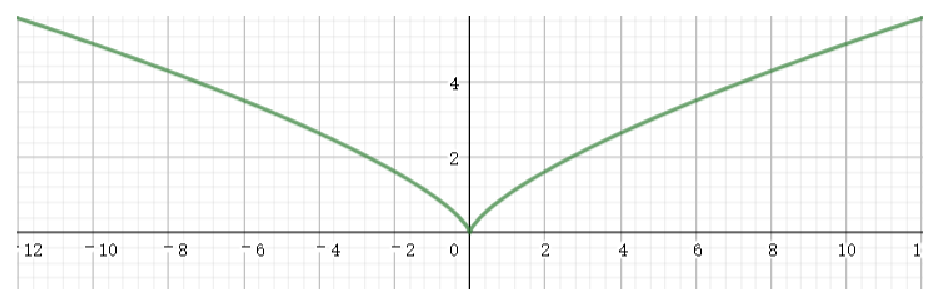
\includegraphics[width=0.5\linewidth]{imgs/quasi.eps}
	}
	\quad
	\subfigure[多模态函数]{
	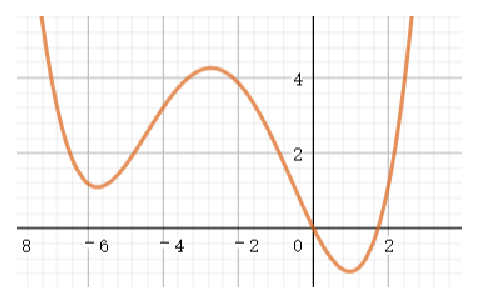
\includegraphics[width=0.25\linewidth]{imgs/multi.eps}
	}
	\caption{拟凸函数又称单模态函数}
\end{figure}

\li{向量长度$ x\in\rs{n} $,x中最后一个非零元素的位置}{
	$f(x)=\bc{
		\max\{i,\ x_i\neq 0\}\quad& x\neq 0\\ 
		0\quad&x>0
	}$\\
	$ S_\alpha=\{f(x)\leq \alpha\}\Rightarrow\ \forall i=\lfloor i\rfloor+1\dots n,\ x_i=0 $\\
	相当于取子空间,一些轴上取零,其余轴上的值任意,为凸集,因此f(x)为拟凸函数
}

\li{线性分数函数$ f(x)=\dfrac{a^Tx+b}{c^Tx+d},\ dom\ f=\{x\mid c^Tx+d>0\} $}{
	$ S_\alpha=\{x\mid c^Tx+d>0,\ \dfrac{a^Tx+b}{c^Tx+d}<\alpha\}=\{x\mid c^Tx+d>0,\ ax+b\leq\alpha(c^Tx+d)\}$\\ [8pt]
	该集合表示一个多面体,为凸集,因此f(x)为拟凸函数
}

\textbf{可微拟凸函数的一阶条件:}\dom{f}为凸,$ \forall x,y\in dom\ f,\ f(y)\leq f(x)\Rightarrow\nabla^Tf(x)(y-x)\leq  0 $\\
\paint[blue]{20中只证明了$\theta\to 1$情况,具体的证明见21(不好描述)}\\
\paint{凸函数的一阶条件告诉我们局部最小即为全局最小:若$ \nabla f^T(x)=0,\ \forall y,\ f(y)\geq f(x) $\\拟凸函数的一阶条件并没有告诉我们什么,若$ \nabla f^T(x)=0,\ \forall y, f(y)\leq f(x)\Rightarrow 0\leq 0 $无意义\\
这也就是凸函数和拟凸函数一阶条件的最大不同,拟凸函数不能保证一阶导数为0的点有意义}

\textbf{可微拟凸函数的二阶条件:}\dom{f}为凸,且$ y^T\nabla f(x)\geq 0\Rightarrow y^T\nabla^2f(x)y\geq 0 $\\
考虑$ n=1 $的情况,$ yf' (x)\geq 0\Rightarrow y^2f''(x)\geq 0 $\\
$ y=0 $时情况成立,当$ y\neq 0 $,只需$ f'(x)=0 $,一定有$ yf' (x)=0\Rightarrow f''(x)\geq 0 $\\
推广到高维情况,即对凸函数而言,所有点的二阶Hessian矩阵半正定,而对于拟凸函数而言,只需要部分关键点,$ f'(x)=0 $这些点半正定\\
\paint{由此可以用该二阶条件判断函数是否是拟凸函数,考虑一阶为0的点二阶是否大于等于0}

\textbf{log concave/log convex:}
\rebacklinespread
\begin{description}[itemsep=0pt,parsep=0pt,topsep=0pt]
	\item[log concave]$ f:R^n\to R $为log concave,若$ f(x)>0,\forall x\in dom\ f$且$ log\,f $为凹函数
	\item[log convex] $ f:R^n\to R $为log convex,若$ f(x)>0,\forall x\in dom\ f$且$ log\,f $为凸函数
\end{description}
\paint{f为凹函数\sune log f为凹函数,f为凸函数 \usne log f为凸函数}\\
可以将f看做$ e^{log\ f} $,利用函数组合的规则理解
\end{document}